\chapter{Estado del Arte}

\section{Colegio Profesional}
Un colegio profesional es, según el artículo primero de la Ley de Colegios Profesionales, una corporación de derecho público, amparada por la ley y reconocida por el Estado, con personalidad jurídica propia y plena capacidad para el cumplimiento de sus fines \cite{colegiosjunta}. \\

La función principal de estas corporaciones es la de velar por el cumplimiento de una buena labor profesional mediante las siguientes acciones:
\begin{itemize}
\item La ordenación del ejercicio de la profesión, dentro del marco legal respectivo y en el ámbito de sus competencias.
\item La representación institucional exclusiva de la profesión cuando estén sujetas a colegiación obligatoria.
\item La protección de los intereses de las personas consumidoras y usuarias de los servicios de sus personas colegiadas.
\item La defensa de los intereses profesionales de las personas colegiadas. \\
\end{itemize}

La creación de un colegio profesional solo es posible cuando se cumplen las siguientes condiciones previas:
\begin{itemize}
\item Existencia de un título académico oficial que respalde el ejercicio de la profesión.
\item Interés público que justifique el carácter colegiado de esa profesión.
\item Petición mayoritaria de los profesionales interesados.  \\
\end{itemize}

La colegiación obligatoria para el ejercicio de una profesión solo será exigible cuando así se establezca por una ley estatal. \\

Los colegios de profesiones técnicas (fundamentalmente ingeniería y arquitectura) visan los trabajos profesionales de sus colegiados. El visado es un acto de control técnico de determinados trabajos que habitualmente está delegado por la Administración mediante una normativa \cite{colegioswikipedia}. El objeto del visado es comprobar, al menos:
\begin{itemize}
\item La identidad y habilitación profesional del autor del trabajo.
\item La corrección e integridad formal de la documentación del trabajo profesional acuerdo con la normativa aplicable al trabajo del que se trate.
\end{itemize}


\section{Colegio Profesional de Ingenieros en Informática de Andalucía}
El Colegio Profesional de Ingenieros en Informática de Andalucía (CPIIA) es, como su propio nombre indica, un Colegio Profesional que regula el ejercicio de los profesionales del ámbito de la Ingeniería Informática en la comunidad de Andalucía. \\

Este se constituyó el 30 de septiembre de 2008, a razón de la necesidad de ordenación de la profesión \cite{cpiia}. Tiene entre sus funciones:
\begin{itemize}
\item La protección de los intereses de los consumidores y usuarios de los servicios de sus colegiados.
\item La elaboración, publicación y actualización de la lista de colegiados como prestadores de servicios profesionales relacionados con la Ingeniería Informática.
\item Elaboración, publicación y vigilancia del cumplimiento del Código Deontológico, en coordinación con el Consejo General de Colegios Oficiales de Ingeniería en Informática (CCII).
\item Ordenación del ejercicio de la profesión de Ingeniero e Ingeniera en Informática, en colaboración con el CCII.
\item Participar en la elaboración de los planes de estudio correspondientes a las titulaciones universitarias vinculadas con el ejercicio de la profesión de Ingeniero en Informática.
\item Velar por el adecuado nivel de calidad de las prestaciones profesionales de las personas colegiadas.
\item Adoptar las medidas necesarias para evitar el intrusismo profesional y la competencia desleal, en colaboración con el CCII.
\item Elaborar una carta de servicios al ciudadano.
\item Contribuir al cambio de modelo productivo, fomentando la industria y el emprendimiento informático, así como la utilización masiva de la informática para aumentar la productividad laboral y la mejora de las relaciones sociales y el disfrute del ocio, en colaboración con el CCII.
\end{itemize}


\section{Turno de Actuación Profesional}
El Turno de Actuación Profesional (TAP) es un servicio destinado a atender las peticiones de trabajo profesional que se realicen por cualquier persona física, organismos y entidades públicas y privadas hacia los profesionales colegiados que voluntariamente figuren inscritos en el mismo, en el ámbito de las actuaciones judiciales, periciales o de auditoría \cite{tapecoourense}. \\

Los TAP son gestionados por Colegios Profesionales. Estos definen individualmente las características de sus propios TAPs, por lo que pueden ser diferentes aquellos gestionados por distintos Colegios, incluso siendo relativos a un mismo campo de trabajo. A pesar de esto, existen una serie de atributos y comportamientos que suelen ser comunes entre ellos \cite{colegiosinformaticaccii}:
\begin{itemize}
\item Los profesionales colegiados son organizados gracias a un conjunto de listas. El número de estas por cada tipo de lista dependerá del Colegio que las gestione, teniendo en cuenta las divisiones territoriales y el número de colegiados y solicitudes. El criterio de ordenación de los profesionales inscritos dentro de las mismas es escogido por el Colegio. La pertenencia a dichas listas es voluntaria y no exclusiva.
\item Los requisitos comunes para pertenecer a alguna de las listas de profesionales incluyen:
	\begin{itemize}
	\item Estar colegiado, en el Colegio Profesional en cuestión, y al corriente del pago de las cuotas colegiales.
	\item No estar cumpliendo sanciones que inhabiliten para el ejercicio de la profesión.
	\item Poseer un título oficial que corresponda a la materia objeto a tratar.
	\item Aceptar expresamente la publicación de sus datos en las listas del TAP.
	\end{itemize}
Además, se suelen establecer otros requisitos específicos, aunque dependen del campo de trabajo.
\item La renovación anual de la solicitud para mantenerse en las listas, en caso de querer permanecer en las mismas. \\
\end{itemize}

En cualquier caso, el incumplimiento del reglamento del TAP puede acarrear la inhabilitación temporal del profesional.


\section{Aplicación a Desarrollar}
Se pretende desarrollar un sistema de gestión de TAP para el CPIIA \cite{reglamentotapcpiia}, que realizará, mediante una serie de listas de profesionales y de revisores, la asignación automática de los TAP. Estas podrán ser creadas por los Responsables, que deberán definir si es de profesionales o revisores, el tipo de la lista, si es pública o privada y el territorio que abarca. El territorio podrá ser una provincia, una región, la comunidad autónoma andaluza a nivel nacional. \\

Las listas de actuación profesional se emplearán para asignar profesionales a aquellas personas que contacten con el CPIIA. En caso de que el profesional al que se le asigne un turno lo rechace exponiendo los motivos, se correrá su turno asignándoselo al siguiente de la lista. Si el Colegio determina que la solicitud no cumple los requisitos necesarios, como puede ser por falta de información, y la declara inválida, esta no será asignada a ningún profesional de la lista. \\

Las listas públicas estarán a disposición del público en la web oficial del Colegio y permitirá a quien lo desee contactar con un profesional concreto directamente. En ella se facilitará información de los profesionales colegiados, como área de especialización, área de cobertura, nombre, apellidos, email, teléfono de contacto, experiencia en el área y URL a la web del profesional en caso de disponer de una. En los proyectos asignados por lista pública no requieren que el colegiado realice ninguna información de seguimiento al Colegio. \\

La ordenación de las listas se realizará por orden alfabético respecto a apellidos y nombres, y los profesionales inscritos en ellas podrán consultar cuantos colegiados le preceden en turno en la misma. \\

Los requisitos para poder inscribirse en estas listas son:
\begin{itemize}
	\item Estar colegiado, y al corriente del pago de las cuotas colegiales.
	\item Tener una titulación de Ingeniero en Informática homologada en territorio español.
	\item No estar cumpliendo sanciones que inhabiliten para el ejercicio de la profesión.
	\item Permitir que sus datos personales sean utilizados para la confección de las listas.
	\item Demostrar que conoce las obligaciones de un profesional y las consecuencias legales.
	\item Declararse conocedor de las obligaciones fiscales.
	\item Estar en posesión de un seguro de responsabilidad civil. \\
\end{itemize} 

Existirá una comisión del TAP, constituida por miembros de las listas de profesionales que lo soliciten y demuestren haber realizado al menos dos proyectos a lo largo de varios años. Esta tendrá la responsabilidad de la composición, gestión y envío de las listas de profesionales. También es responsable de interpretar y aplicar el reglamento, sancionando a los profesionales que lo incumplan, pudiendo estos ser expulsados de las listas por un tiempo determinado. \\

El sistema contará con tres perfiles de usuarios, que son los siguientes:
\begin{itemize}
	\item Usuario, que hace referencia a cualquier persona que no esté colegiada.
	\item Colegiado, que define a cualquier miembro que haya sido registrado en el sistema y tenga asignado un número de colegiado.
	\item Responsable, es aquel colegiado que tiene otros permisos para la administración del sistema. \\
\end{itemize}


Estos perfiles obedecerán una jerarquía, que se puede observar en la \textbf{\hyperref[fig:jerarquiaPerfiles]{Figura 2.1}}, de tal manera que las funciones propias de los Usuarios también serán realizables por los Colegiados y los Responsables. De igual manera, las funciones que se le permiten ejecutar a los Colegiados son accesibles para los Responsables.

\begin{figure}[!htbp]
  \centering
  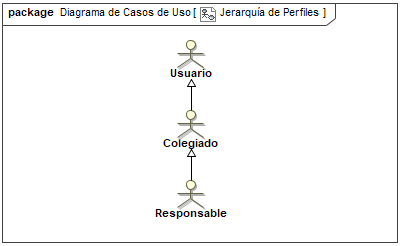
\includegraphics{JerarquiaPerfiles.png}
  \caption{Jerarquía de Perfiles}
  \label{fig:jerarquiaPerfiles}
\end{figure}
\FloatBarrier

Con el desarrollo e implantación de la aplicación, que cumplirá con lo mencionado anteriormente, se pretende liberar al CPIIA del esfuerzo que supone llevar una serie de TAPs para todos los territorios que contempla y las diferentes especialidades del ámbito de la ingeniería informática.


\section{Aplicación de las Competencias Existentes en el Mercado}
Múltiples colegios profesionales cuentan con sistemas de gestión de turnos de actuación profesional. Pero la situación antes la que nos encontramos es que no existe un software genérico que permita gestionar este apartado, siendo necesario el desarrollo de soluciones a medida para cada uno de estos. Además, las soluciones que tienen estos son privadas y cerradas, restringiendo el acceso a usuarios que no formen parte de sus listas. Por esta última razón, no ha sido posible compararlas con la aplicación que se pretende desarrollar.
